\section{Theoretical Analysis} \label{sec:analysis}
 


\subsection{Gain Stage}



\begin{equation}
 \begin{cases}
 \frac{vo}{vi}=\frac{g_{m2}}{g_{\pi 2}+g_O+g_{o2}+g_{m2}}\\
  Z_{I2}=\frac{g_{\pi 2}+g_O+g_{o2}+g_{m2}}{g_{\pi 2}(g_O+g_{o2}+g_{m2})}\\
  Z_{02}=\frac{1}{g_{\pi 2}+g_O+g_{o2}+g_{m2}}
 \end{cases}
\end{equation}

where $g_{\pi 2}$ is the input incremental conductance, $g_{o 2}$ and $g_O$ is the $R_O$'s conductance


The results are shown in the following table.

\begin{table}[!htb]
\centering
  \begin{tabular}{|c|c|}
    \hline    
    {\bf Parameter} & {\bf Value} \\ \hline
    \input{../mat/outputstage.tex}
 \end{tabular}
 \caption{Results Output Stage}\label{tab:outputstage}
\end{table}
 with capacitance, as we can see in the picture bellow.
 
 \begin{figure}[h] \centering
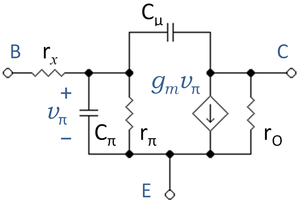
\includegraphics[width=0.4\linewidth]{transistor.png}
\vspace{-3mm}
\caption{Transistor incremental model with capacitance}\label{fig:rc}
\end{figure}



\newpage
